\section{Experiments}
\label{sec:results}
We run experiments on maps from the GPPC 2012 benchmarks~\cite{sturtevant2012benchmarks},
including 105 game maps and 6 artificial maps - 2 out of 9 maps each in \textit{mazes, rooms, random}.
Although all forward CPDs and most of reverse-centroid CPDs work on the rest of the 21 artificial maps, 
they are too large to build the full reverse CPD, so that they are excluded to avoid dealing with 
missing values.
%\footnote{due to the memory limit we excluded artificial maps larger than 400 $\times$ 400.}
All algorithms are implemented in {\tt C++} and compiled with {\tt -O3} flag.
We use the following abbreviations for convenience:
\begin{itemize}
    \item $\tt fwd_\delta$: forward CPD with centroid size $\delta$ 
    \item $\tt rev_\delta$: reverse CPD with centroid size $\delta$
\end{itemize}
Note that $\delta = 0$ means the full forward or reverse CPD.
We used proximity wildcards for all forward CPDs, but not for reverse CPDs where they did not lead to any compression.
Our test machine is {\tt \small Linux 4.19.45-1-MANJARO} with {\small \tt i5-8600 CPU @ 3.10GHz} CPU and {\tt 15GB} memory.

\begin{figure}
    \centering
    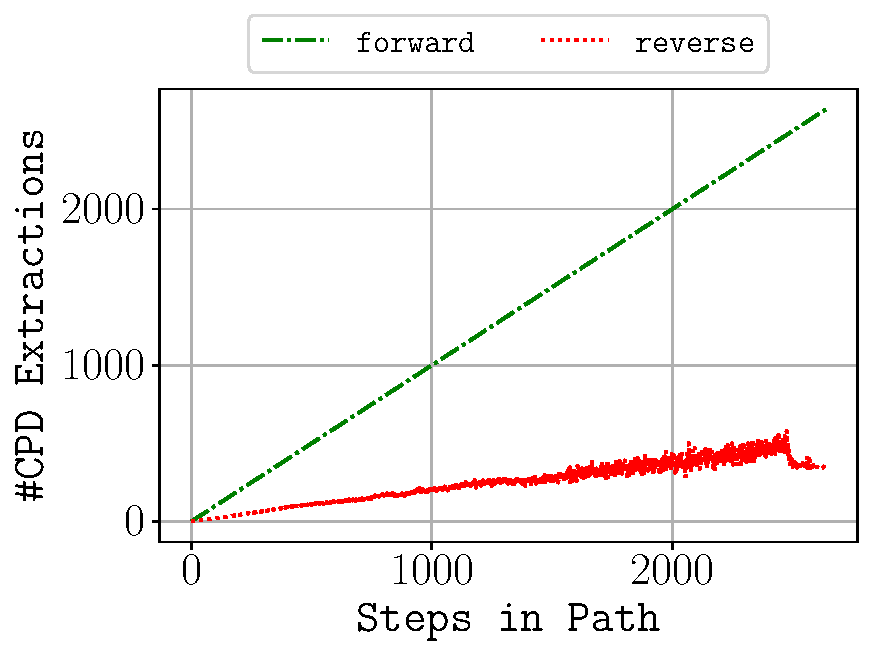
\includegraphics[width=\columnwidth]{pic/steps-access.pdf}
    \caption{ 
    The number of CPD extractions required to compute a path averaged over 
    all queries (1087778 in total) across 111 maps, with $\delta=0,2,4,8,16,32,64$.}
    \label{fig:access}
\end{figure}


\subsection{Experiment 1: Size of CPDs}

\begin{figure}
    \centering
    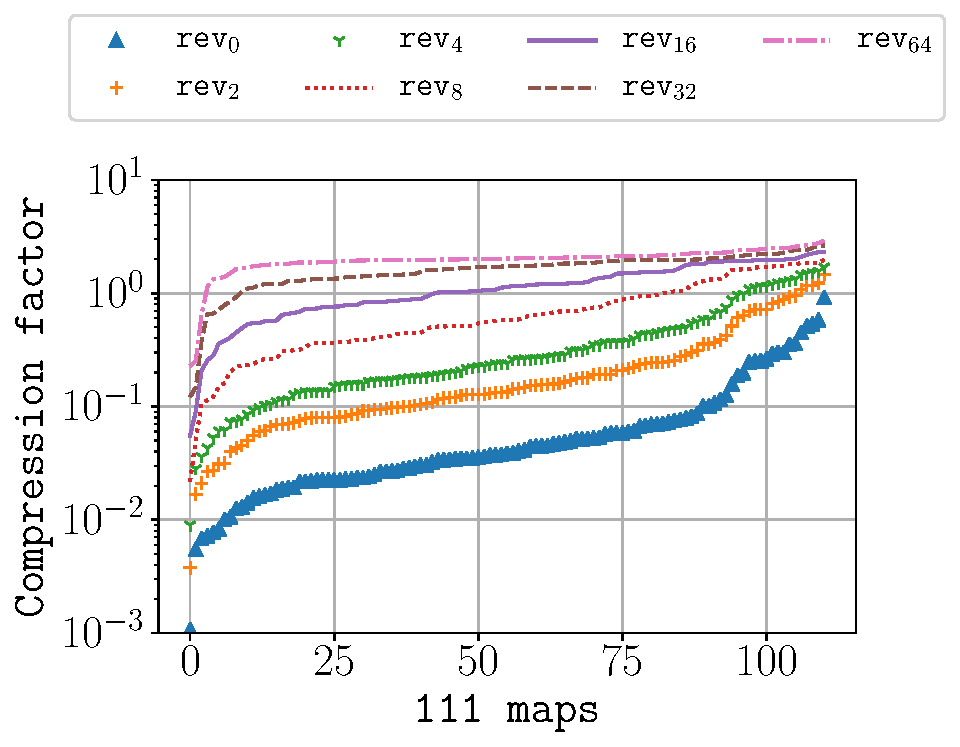
\includegraphics[width=\columnwidth]{pic/fwd-bwd.pdf}
    \caption{
    Ratio of CPD size between forward and reverse, $ratio=\frac{|\tt fwd_\delta|}{|\tt rev_\delta|}$,
    sorted from smallest to largest, with $\delta = 2,4,8,16,32,64$.}
    \label{fig:fwd-bwd}
\end{figure}

%\begin{table}[tb]
%    \centering
%    \begin{tabular}{lrr}
%    \toprule
%    {} &      $\delta=32$ &      $64$ \\
%    \midrule
%    mean  &    1.66 &    2.02 \\
%    min   &    0.12 &    0.23 \\
%    median&    1.73 &    2.02 \\
%    max   &    2.64 &    2.91 \\
%    \bottomrule
%    \end{tabular}
%    \label{tab:size-summary}
%\end{table}
%

In this experiment, we examine the compression of forward CPDs and reverse
CPDs with different $\delta$.
To show results, we define $\tt ratio_{\delta}=\frac{|\tt fwd_{\delta}|}{|\tt
rev_{\delta}|}$, where $|\tt rev_{\delta}|$ is the size of reverse CPD,
and $|\tt fwd_{\delta}|$ is the size of forward CPD.
Figure~\ref{fig:fwd-bwd} shows $\tt ratio_{\delta}$ with $\delta =
0,2,4,8,16,32,64$.
Note that when $\delta=32,64$, the reverse CPD outperforms forward CPD in
most maps --- $ratio_{32}$ ($ratio_{64}$) is more than $1.73$ ($2.02$)
in more than $50\%$ of maps and up to $2.64$ ($2.91$).

%\begin{table*}[]
%    \centering \small
%    \begin{tabular}{ll|rrrrrrr}
%        Map     & stat & $\delta =0$ & 2 & 4 & 8 & 16 & 32 & 64 \\ \hline 
%\tt  Aurora       & C & 493772 & 129509 & 64429& 18485& 6405 & 1981 & 697 \\
%                  & T & 764.90 &200.62  &99.80 &28.65 & 9.92 & 3.07 & 1.08 \\ 
%                  & F & \bf 342.28 & \bf 305.91 & \bf 223.91 &  \bf 147.19 &   \bf 97.65 &   63.02 &   45.25\\
%                  & P & NaN      &  9771.73 &  4860.59 & 1384.69  & 476.22 & 143.81      & 47.07  \\
%                  & R & 10162.89 &  2663.07 &  1326.78 &   380.87 &   133.77 & \bf 43.40 & \bf 17.07\\ \hline
%\tt orz103d       & C &  40392 &   11411 &   5468 &   1928 &   723 &   249 &  111 \\
%                  & T &  2.56  & 0.72    & 0.35   & 0.12   & 0.05  & 0.02  & 0.01 \\
%                  & F & \bf 1.48 & \bf 1.58 & \bf 1.52 & \bf 1.46 & \bf 1.40 &  \bf 1.34 &    1.30 \\
%                  & P & 503.80 & 142.72   & 68.67    & 24.53    & 9.51     & 3.60     & 1.87 \\
%                  & R & 179.06 &    51.00 &    24.69 &     9.03 &     3.69 &     1.59 & \bf 0.98\\ \hline
%\tt maze-400-4    & C & 127996 & 40000 & 16143 & 6302 & 2343 & 995 & 431\\
%                  & T & 37.94  &11.86  & 4.79  & 1.87 & 0.69 & 0.29& 0.13\\
%                  & F & \bf 4.16 & \bf 4.57 & \bf 4.42 & \bf 4.21 & \bf 4.00 & \bf 3.85 & \bf 3.71 \\
%                  & P & 7909.59  & 2473.07  & 998.97   & 390.93   & 146.32   & 63.02    & 28.17 \\
%                  & R & 3883.68 & 1214.90 & 491.22  & 192.70 & 72.61 & 21.72 & 14.61 \\ \hline
%\tt room-400-40   & C & 152811 & 40000 & 18325 & 4980 & 1660 & 472 & 130\\
%                  & T & 60.46  & 15.83 & 7.25  & 1.97 & 0.66 & 0.19& 0.05\\
%                  & F & \bf 74.40 & \bf 67.12 & \bf 44.90 & \bf 29.66 & \bf 20.07 & 12.63 & 8.48 \\
%                  & P & 3190.34 & 836.35 & 384.35 & 105.75& 36.49    & 11.78 & 4.51 \\
%                  & R & 2161.59 & 567.15 & 260.68 & 72.23 & 25.30 & \bf 8.57 & \bf 3.64 \\ \hline
%\tt random-400-33 & C & 103535 & 40792 & 20640 & 9023 & 3844 & 1827 & 860 \\
%                  & T & 24.18  & 9.53  & 4.82  & 2.11 & 0.90 & 0.43 & 0.20\\
%                  & F & \bf 41.14 & \bf 35.34 & \bf 29.97 & \bf 23.64 & \bf 18.12 & \bf 14.09 & \bf 10.32 \\
%                  & P & NaN     & 6408.98 & 3243.44 & 1418.59& 605.10 &288.30 & 136.44 \\
%                  & R & 5323.83 & 2098.43 & 1062.38 & 465.17 & 198.86 & 95.15 & 45.45 \\ \hline
%    \end{tabular}
%    \caption{Number of (C)entroids, building (T)ime in minutes, and memory requirements MB for (F)orward, 
%    %(P)urely backward CPDs 
%    and improved (R)everse CPDs for 
%    different radii of centroids on a number of example maps. Note that for $\delta = 0$ the number of centroids in the number of cells in the map.}
%    \label{tab:sizes}
%\end{table*}

\begin{table*}[bt]
    \centering \scriptsize
\begin{tabular}{ll|r@{~}rr@{~}rr@{~}rr@{~}rr@{~}rr@{~}rr@{~}r}
\toprule
       &$\delta$& \multicolumn{2}{c}{0} & \multicolumn{2}{c}{2} & \multicolumn{2}{c}{4} & \multicolumn{2}{c}{8} & \multicolumn{2}{c}{16} & \multicolumn{2}{c}{32} & \multicolumn{2}{c}{64} \\
\midrule
       map &stat& F     &     R         & F     &    R          & F         &    R      & F     &   R           & F         &   R        & F        &   R         & F           &   R\\
\midrule
 \tt  Aurora &C &\multicolumn{2}{c}{493772}&\multicolumn{2}{c}{129509}&\multicolumn{2}{c}{64429}&\multicolumn{2}{c}{18485}&\multicolumn{2}{c}{6405}&\multicolumn{2}{c}{1981}&\multicolumn{2}{c}{697}\\ 
             %&T &  119.80 &  \textbf{119.12 }&  106.63 & \textbf{ 27.87 }&  105.80 & \textbf{ 13.62 }&  105.52 & \textbf{ 3.92} &  105.30 & \textbf{ 1.37 }&  105.16 & \textbf{ 0.42 }&  105.25 &  \textbf{0.14 }\\
             &T &  790.03 &  831.18&  207.21 & 218.00 &  103.09 & 108.46 & 29.58 & 31.12& 10.25 & 10.78 & 3.17 & 3.33 & 1.12 & 1.17 \\
             &M & \textbf{342.28 } &10162.89 & \textbf{305.91 } &2663.07 & \textbf{223.91 } &1326.78 &\textbf{ 147.19 } &380.87 &\textbf{ 97.65 }  & 133.77& 63.02 & \textbf{43.40 }& 45.25   & \textbf{17.07} \\ \hline
             
 \tt    orz103d &C &\multicolumn{2}{c}{40392}&\multicolumn{2}{c}{11411}&\multicolumn{2}{c}{5468}&\multicolumn{2}{c}{1928}&\multicolumn{2}{c}{723}&\multicolumn{2}{c}{249}&\multicolumn{2}{c}{111}\\ 
            %&T &    0.51 &    \textbf{0.50 }&    0.50 &  \textbf{ 0.14 }&    0.50 &  \textbf{ 0.07 }&    0.49 &  \textbf{0.03 }&    0.49 &  \textbf{0.01 }&    0.49 &  \textbf{0.00 }&    0.49 &  \textbf{0.00 }\\
             &T &    2.69 &    3.37   &  0.76 & 0.95 &  0.37 & 0.46 & 0.13 & 0.16 & 0.05 & 0.06 & 0.02 & 0.02 & 0.01 & 0.01 \\
             &M & \textbf{1.48}   & 179.06  & \textbf{1.58}   & 51.00  & \textbf{1.52}   & 24.69  & \textbf{1.46}   & 9.03  & \textbf{1.40 }   & 3.69  & \textbf{1.34 }   & 1.59  & 1.30    & \textbf{0.98} \\ \hline
             
\tt maze-400-4 &C &\multicolumn{2}{c}{127996}&\multicolumn{2}{c}{40000}&\multicolumn{2}{c}{16143}&\multicolumn{2}{c}{6302}&\multicolumn{2}{c}{2343}&\multicolumn{2}{c}{995}&\multicolumn{2}{c}{431}\\ 
            %&T &    5.66 &  \textbf{5.65}&    5.46 &  \textbf{1.73}&    5.40 & \textbf{0.70}&    5.33 & \textbf{ 0.27 }&    5.32 & \textbf{0.10}&    5.30 &  \textbf{0.05 }&    5.31 &  \textbf{0.02}\\
             &T &   40.53 & 44.80 & 12.67 & 14 & 5.11 & 5.65 &  2.00  & 2.21 & 0.74 & 0.82 &  0.32 & 0.35 & 0.14 & 0.15\\
             &M & \textbf{4.16}  & 3883.68 &  \textbf{4.57}  & 1214.90& \textbf{4.42}   & 491.22 & \textbf{4.21 }   & 192.70& \textbf{4.00 }   & 72.61 &\textbf{3.85}   & 21.72 & \textbf{3.71}   & 14.61 \\ \hline

\tt room-400-40 &C &\multicolumn{2}{c}{152811}&\multicolumn{2}{c}{40000}&\multicolumn{2}{c}{18325}&\multicolumn{2}{c}{4980}&\multicolumn{2}{c}{1660}&\multicolumn{2}{c}{472}&\multicolumn{2}{c}{130}\\ 
            %&T &    9.40 &    9.40 &    9.45 &   \textbf{2.49} &    9.41 &  \textbf{ 1.11} &    9.38 &  \textbf{0.31} &    9.35 & \textbf{ 0.11} &    9.33 &  \textbf{0.03} &    9.33 &  \textbf{0.01} \\
             &T &  63.67 & 66.22 & 16.67 & 17.33 & 7.64 & 7.94 & 2.08 & 2.16  & 0.69 & 0.72 & 0.20 & 0.21 & 0.05 & 0.06 \\
             &M &  \textbf{74.40 } & 2161.59 & \textbf{67.12}   & 567.15 & \textbf{44.90}   & 260.68 &\textbf{ 29.66 }  & 72.23 & \textbf{20.07 }  & 25.30 & 12.63  & \textbf{8.57 } & 8.48    & \textbf{3.64} \\ \hline
             
\tt random-400-33&C &\multicolumn{2}{c}{103535}&\multicolumn{2}{c}{40792}&\multicolumn{2}{c}{20640}&\multicolumn{2}{c}{9023}&\multicolumn{2}{c}{3844}&\multicolumn{2}{c}{1827}&\multicolumn{2}{c}{860}\\ 
            %&T &    5.36 &    5.36 &    4.94 &   \textbf{1.99} &    4.81 &   \textbf{1.01 }&    4.74 &  \textbf{0.44} &    4.71 &  \textbf{0.19 }&    4.71 &  \textbf{0.09 }&    4.72 &  \textbf{0.05} \\
             &T &  25.88 & 34.51 &  10.20  & 13.60 & 5.16 & 6.88 &2.26 & 3.01 & 0.96 & 1.28 & 0.46 & 0.61  & 0.22  & 0.29\\
             &M & \textbf{41.14 }  & 5323.83 & \textbf{35.34 }  & 2098.43& \textbf{29.97 }  & 1062.38& \textbf{23.64}   & 465.17& \textbf{18.12}   & 198.86& \textbf{14.09}   & 95.15 & \textbf{10.32}   & 45.45 \\

\bottomrule
\end{tabular}
    \caption{Number of (C)entroids, building (T)ime in minutes, and (M)emory requirements in MB for (F)orward and improved (R)everse CPDs for different radii of centroids on five representative maps.
    Note that for $\delta=0$ the number of centroids is the number of cells in the map.}
    \label{tab:cpdinfo}
\end{table*}

We choose 5 representative maps to inspect. Table~\ref{tab:cpdinfo} shows
for the different maps the number of centroids for given radius $\delta$,
the time to construct the forward and the reverse CPDs, and the size of the
forward and the reverse CPDs for this set of centroids.
We note that the time to construct the forward CPDs is similar to that
for the reverse CPDs since both are dominated by the Dijkstra
search time, but faster because it avoids the complication of
``illegal'' move processing.

Compared to a full CPD, the use of centroids reduces the CPD construction time by up to three orders
of magnitude. This is a massive improvement compared to previous work, which has been limited to 
full CPDs.
%
Examining the time we see a scaling with the number of centroids, which
is unsurprising since the main cost is directly proportional to this.

Figures~\ref{fig:fwd0-fwdc},~\ref{fig:fwd-bwd} reflect all the improvements  discussed in this paper. 
We can additionally report (not in Table~\ref{tab:cpdinfo}) that 
without \textit{illegal move} encoding, reverse CPDs can be 1.5 times 
larger than the current version on maps like
\texttt{room-400-40} and \texttt{maze-400-4}, and on other maps 
this simplest version of reverse CPDs can be up to 3 times larger.

Full reverse CPDs can be \emph{orders of magnitude} larger than full forward CPDs
($\delta = 0$). As we increase $\delta$, the reduction in size of forward CPDs is often limited, while the
reduction in size of reverse CPDs is proportional to
the reduction in the number of centroids. Clearly for some maps (\texttt{maze-400-4},
\texttt{random-400-33}) the reverse CPD is prohibitively large, and even a
radius of 64 does not lead to a smaller reverse CPD than the full forward
CPD. For these kinds of maps reverse CPDs are not worthwhile.  For the
remainder of the experiments, we restrict attention to game maps where
reverse CPDs are usually worthwhile.


\subsection{Experiment 2: Path Extraction}
In this experiment, we examine the efficiency and suboptimality 
of the reverse CPD ($\delta=32,64$) in path extraction, 
and compare it with two suboptimal pathfinding algorithms:
\begin{itemize}
    \item {\tt TC}: \textit{Tree Cache}~\cite{k-tc-12},
    a very fast \textbf{unbounded-suboptimal} algorithm based on spanning tree.
    \item {\tt FS$_{\delta_2}$}: \textit{Focal Search}~\cite{DBLP:journals/pami/PearlK82},
    a \textbf{bounded-suboptimal} variant of {\tt A$^*$},
    which guarantees that the difference between length of founded path and optimal path is not greater than a given parameter $\delta_2$. We let $\delta_2 = 2 \delta$ for a fair comparison.
\end{itemize}
We run all scenarios on all game maps from the benchmark set (105 in total).
To examine speed, we run all queries (142534 in total) 5 times and aggregate by mean 
to eliminate random noise.

\begin{table}[bt]
    \centering
    \begin{tabular}{lrrrrr}
    \toprule
    {}               &    mean &     std &   min &median &     max \\
    \midrule
    ${\tt rev}_{32}$       &   14.40 &   13.81 &  0.00 & 10.10 &   64.00 \\
    ${\tt FS}_{64}$        &    5.95 &   10.12 &  0.00 &  0.82 &   63.99 \\ \hline
    ${\tt rev}_{64}$       &   25.62 &   25.96 &  0.00 & 16.83 &  127.80 \\
    ${\tt FS}_{128}$       &   13.22 &   18.71 &  0.00 &  4.97 &  127.99 \\ \hline
    {\tt TC}               &  143.10 &  291.16 &  0.00 & 46.53 & 3194.47 \\
    \bottomrule
    \end{tabular}
    \caption{
    \small
    Suboptimality comparison, 
    evaluated by the difference between 
    the length of an optimal path and the extracted path.}
    \label{tab:diff}
\end{table}

We evaluate suboptimality by \textit{diff}, that is, 
the length of the extracted path minus 
the length of an optimal path.
Table~\ref{tab:diff} shows summaries of \textit{diff} for different approaches.
We can see that the \textit{diff} for the unbounded-suboptimal approach {\tt TC} 
is prohibitively large; 
and {\tt FS} has smaller \textit{diff} than reverse CPDs, 
but still within the same order of magnitude.

\begin{table}[tb]
    \centering
    \begin{tabular}{lrrrrr}
    \toprule
    {}                &   min &    25\% &    50\% &    75\% &  max \\
    \midrule
     ${\tt rev}_{32}$ & 0.003 &  1.447 &  1.980 &  2.532 &  19.777 \\
     ${\tt rev}_{64}$ & 0.016 &  1.431 &  1.960 &  2.526 &  22.901 \\
    %${\tt fwd}_{32}$ & 0.025 &  1.032 &  1.125 &  1.299 &  25.795 \\
    %${\tt fwd}_{64}$ & 0.019 &  1.033 &  1.144 &  1.341 &  21.639 \\
      ${\tt FS}_{64}$ & 0.000 &  0.000 &  0.001 &  0.045 &   4.675 \\
     ${\tt FS}_{128}$ & 0.000 &  0.000 &  0.002 &  0.049 &   4.536 \\
             {\tt TC} & 0.005 &  4.534 &  5.914 &  7.896 &  77.501 \\
    \bottomrule
    \end{tabular}
    \caption{
    Speedup, path extraction time divided by path  extraction time using ${\tt fwd}_0$. A ratio
    greater than $1.0$ means faster.}
    \label{tab:speed}
\end{table}

We evaluate the path extraction speed by time cost \textit{factor},
that is, the path extraction time divided by time cost of ${\tt fwd}_0$.
Table~\ref{tab:speed} shows five number summaries of the time cost factor
of these approaches. Reverse CPDs are nearly twice as fast as
forward CPDs, and Tree Cache is around five times faster, while Focal Search
is orders of magnitude slower due to the requirement to search for paths.

The actual run time on average is that, 
reverse CPDs path extraction cost $7359.29$ ns in total and $19.99$ ns per step,
while forward CPDs cost $14064.18$ ns in total and $30.81$ ns per step,
Tree Cache costs $2564.52$ ns in total and $4.7$ ns per step, and 
Focal Search costs $6.59*10^7$ ns in total and $9.25*10^4$ ns per step.

Based on results above, it is clear that ${\tt rev}_{32}$ and ${\tt
rev}_{64}$ are better for path extraction in terms of tradeoff between
suboptimality and extraction time.  Each of the other competitors is either
bad in terms of suboptimality (\textit{Tree Cache}) or has very slow path
extraction (\textit{Focal Search}).
